Despite the continuous evolution of national cybercrime since the inception of data collection,
along with changes in policies, legal frameworks, and population demographics,
we can create a global cybercrime hotspot map by leveraging crime data recorded by VERIS over the years.
This not only facilitates the analysis of cybercrime volumes by country
but also allows for fitting the data against policy and population variables to assess their influence on cybercrime trends.
\subsection{Cybercrime distribution across the globe}\label{subsec:Building-the-hotspot-map} %3.1
	We made use of a world-wide map to represent all cybercrime occurred around the world.
	In the map, the color filled in each country represents the total number of cybercrime incidents recorded since the beginning of the statistics.
	The color gradient, ranging from dark blue to dark red, corresponds to eight severity levels (1 to 8).
	Countries marked in blue indicate a low frequency of cybercrime incidents, while those marked in red represent a high density of such incidents.
	For instance, the United States, where the VERIS concept was first proposed, has the highest number of recorded incidents (7,236),
	whereas many other countries have only 1 or 2 recorded incidents.
	To address this significant disparity in data distribution, we applied a logarithmic transformation to the data using the formula
	\[ y=\log(1+D_i) \].
	This transformation was implemented using the function
	\[ np.log1p() \]
	in Python to ensure computational precision and stability, particularly for small values.
	The final results are visualized in Figure 1.
	\begin{figure}[htbp]
		\centering
		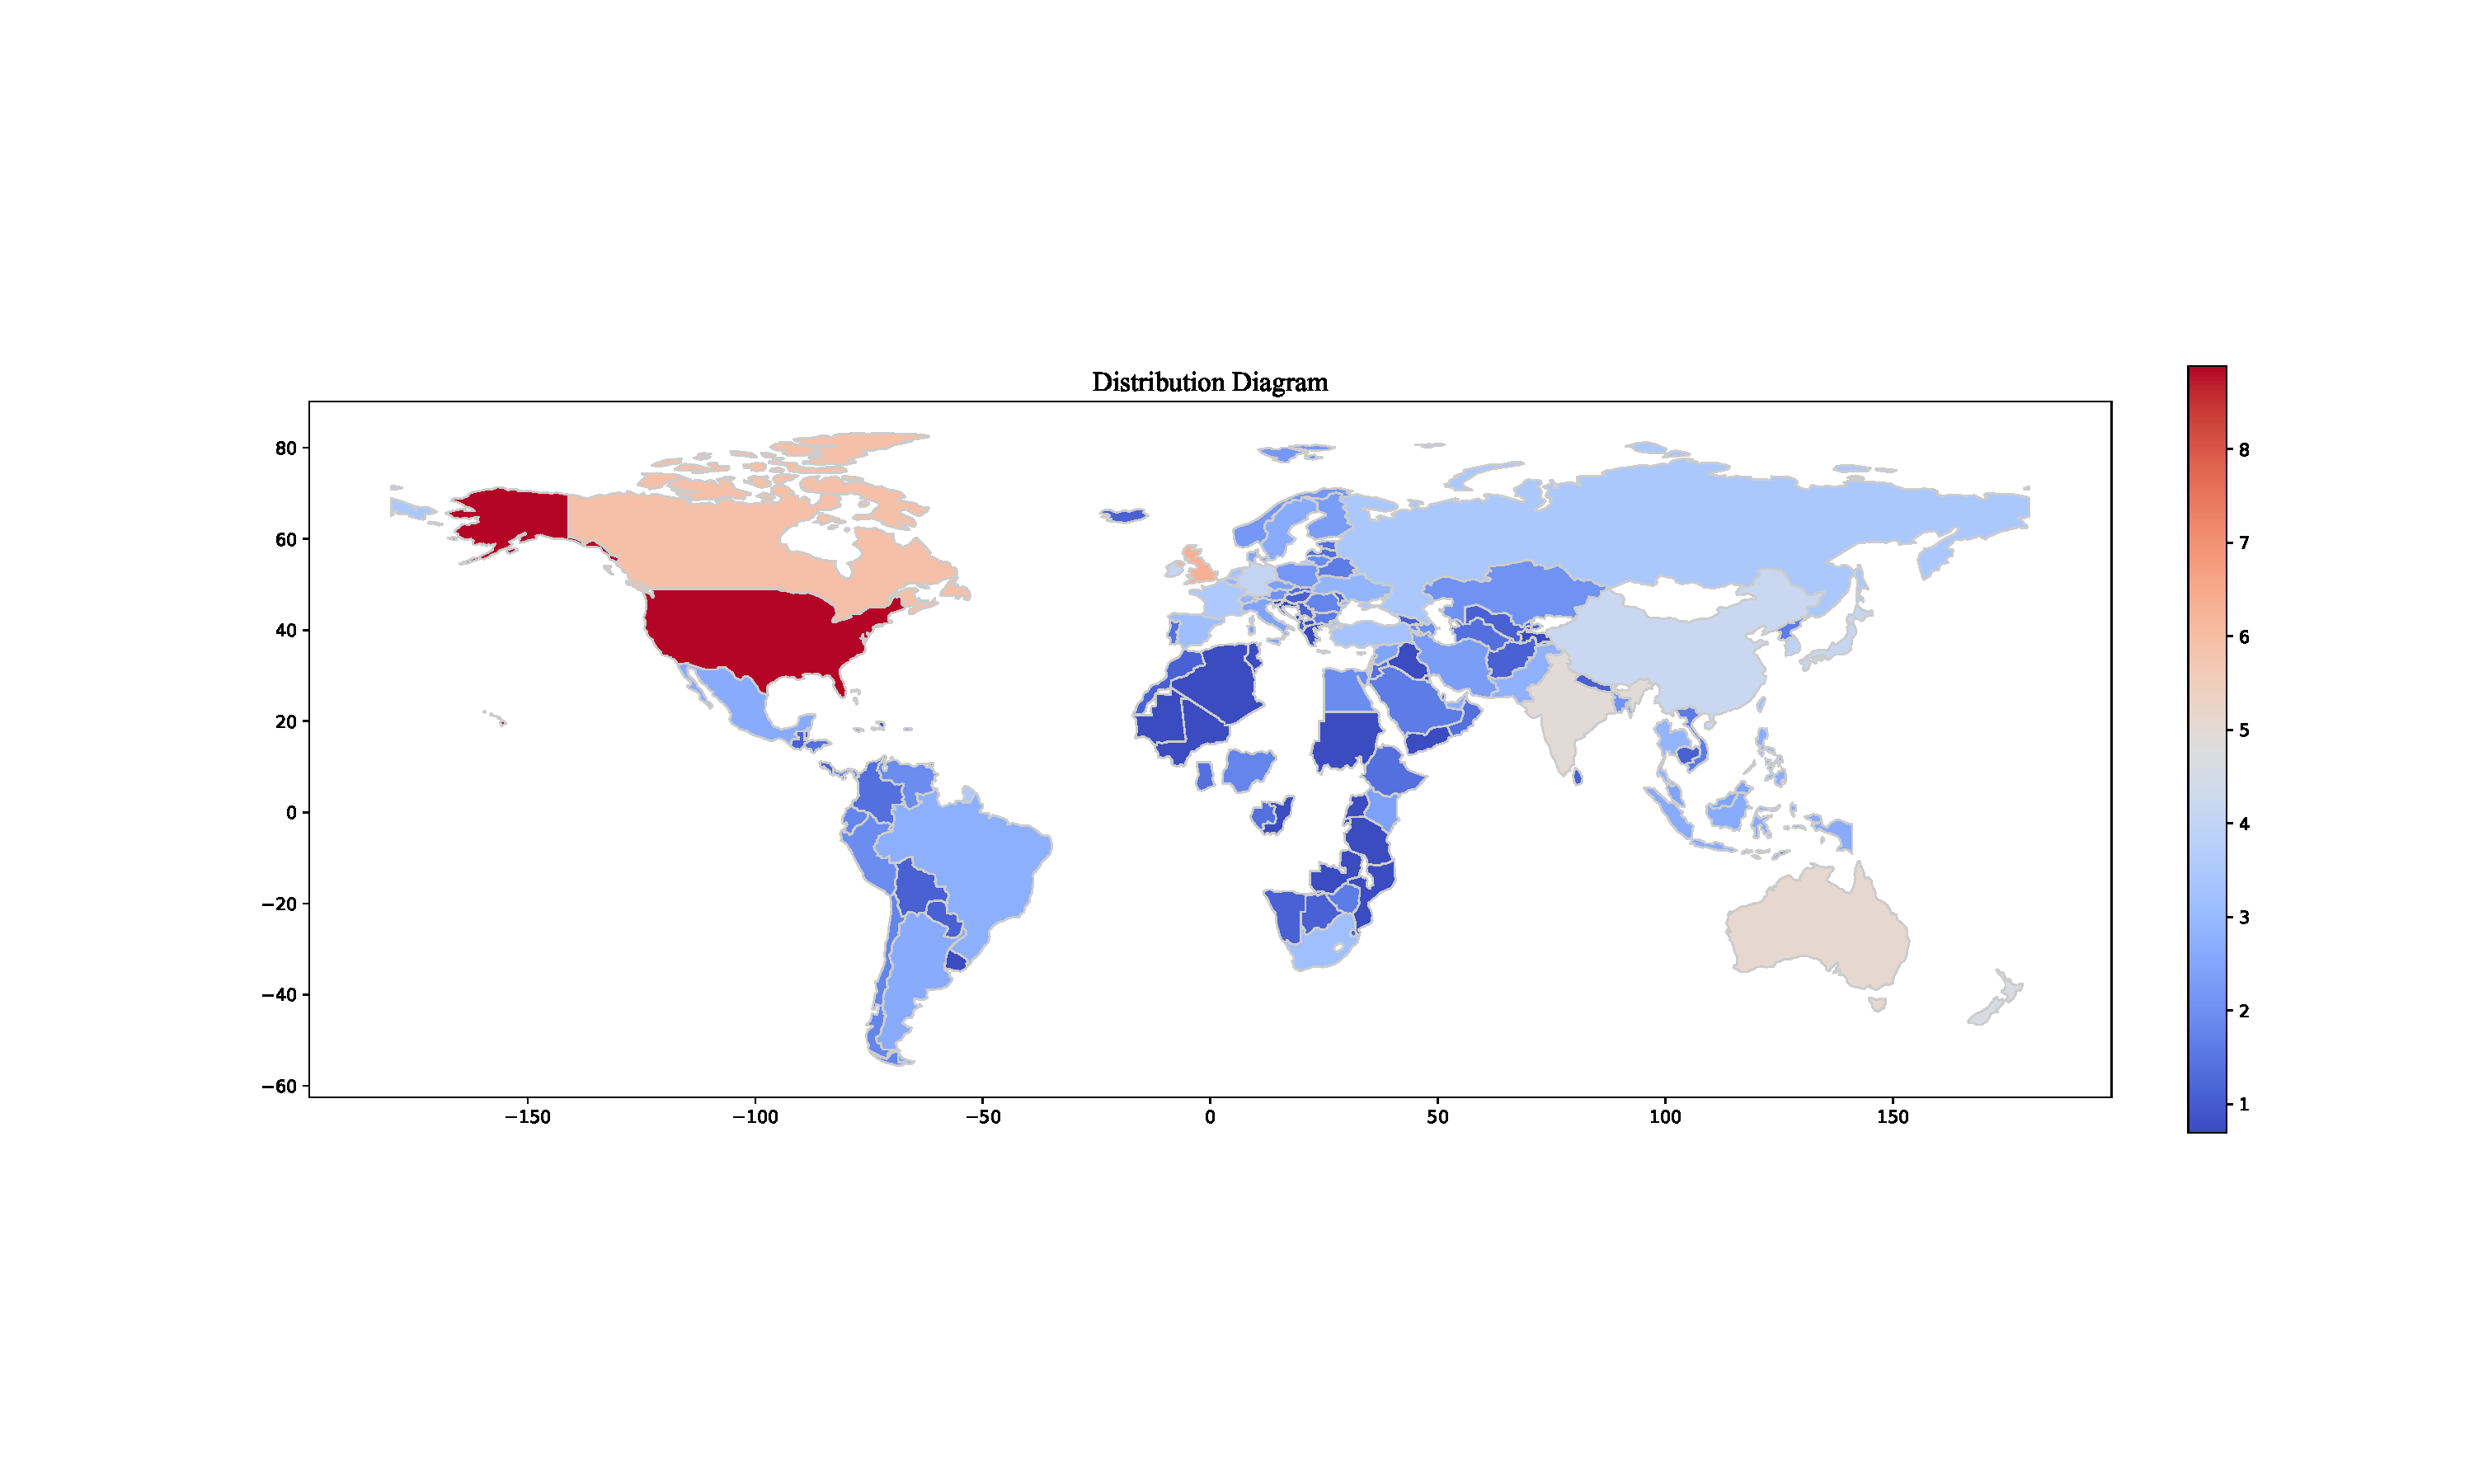
\includegraphics[width=1\textwidth]{./rsrc/Crime_distribution}
		\caption{Crime distribution}\label{fig:crime-distribution}
	\end{figure}
\subsection{High-prevalence regions}\label{subsec:high-prevalence-regions} %3.2
TODO %TODO: 3.2 paragraph
\subsection{Other Cybercrime Incidents}\label{subsec:other-cybercrime-incedents} % 3.3
	Using additional data obtained from the VCDB,
	we constructed heatmaps on a global scale based on the number of successful cybercrimes, thwarted cybercrimes, and reported cybercrimes, respectively.
	Due to the disproportionately high volume of data from the United States,
	we applied the same logarithmic transformation (\( y = \log(1 + D_i) \)) as in Figure~\ref{fig:crime-distribution} for consistency,
	resulting in the three sub-figures presented in Figure~\ref{fig:other-cybercrime-incidents}.

	In sub-figure (a), the number of successful attacks closely aligns with the total number of attacks in most countries.
	For instance, the United States recorded 7,189 successful attacks out of 7,236 total attacks,
	yielding a success rate of \( \frac{7189}{7236} \approx 99.35\% \).
	Similarly, the United Kingdom reported 569 successful attacks out of 574 total attacks,
	with a success rate of \( \frac{569}{574} \approx 99.13\% \).

	In contrast, countries with lower attack volumes did not show significant differences between the total number of attacks and the number of successful attacks,
	indicating that almost every attempted attack was successful.

	In sub-figure (b), only the United States and Canada reported thwarted attack cases, with 6 and 2 instances, respectively.

	In sub-figure (c), the number of successfully reported attacks and the number of countries involved were significantly higher than in sub-figure (b).
	This suggests that while many attacks were successful, a portion of them were detected and reported.
	\begin{figure}[htbp]
		\centering
		\subfigure[Successful Cybercrime Incidents]{
			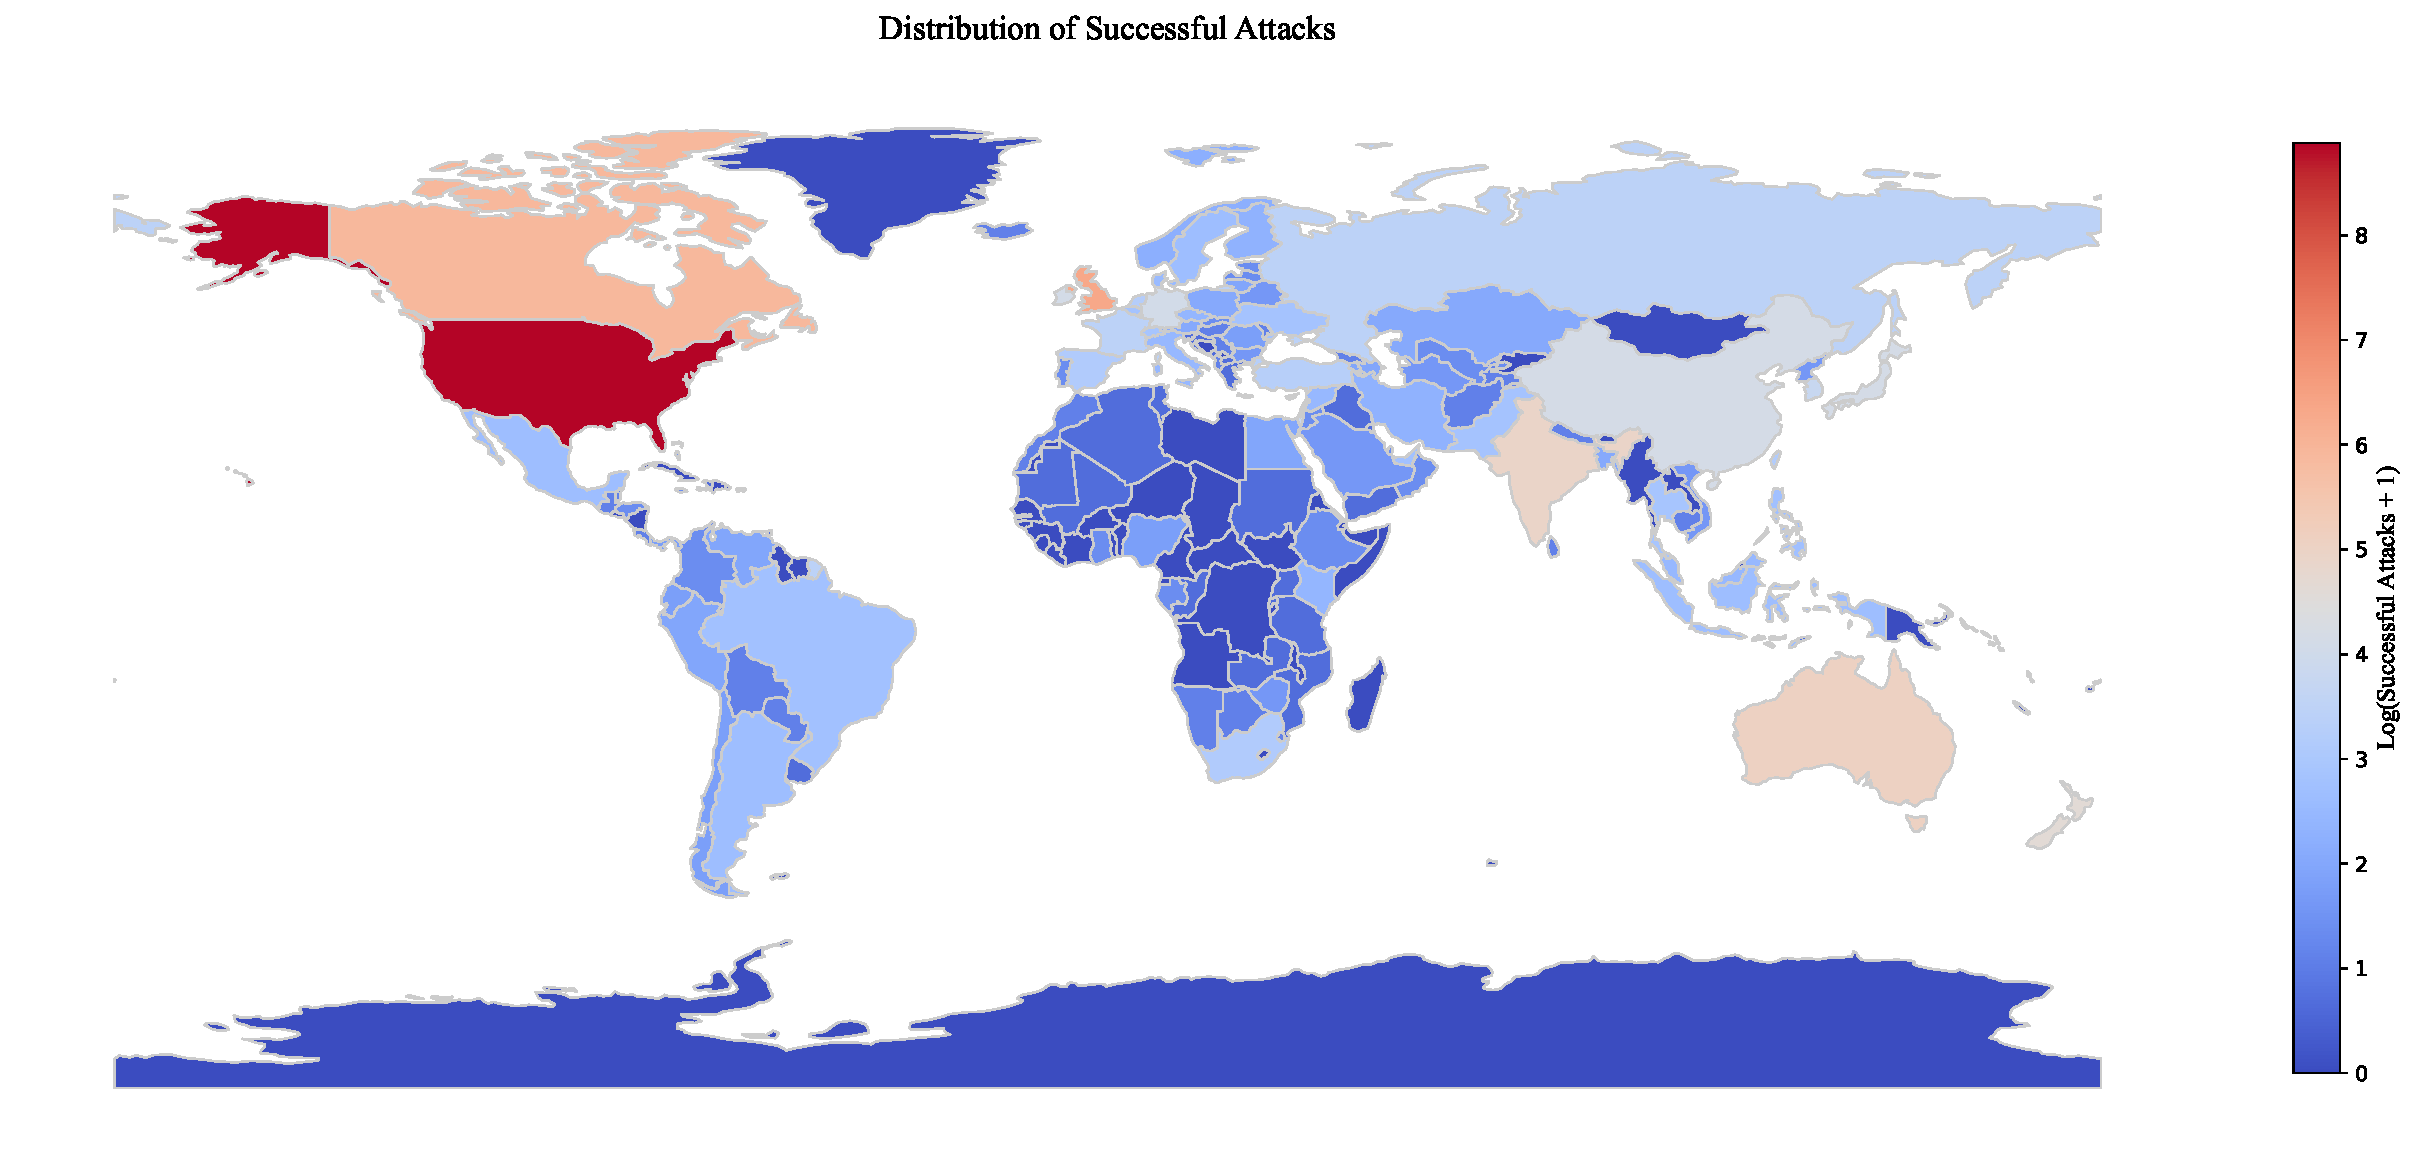
\includegraphics[scale=0.33]{./rsrc/Crime_Successful_distribution}
		}
		\quad
		\subfigure[Mitigated Cybercrime Attempts]{
			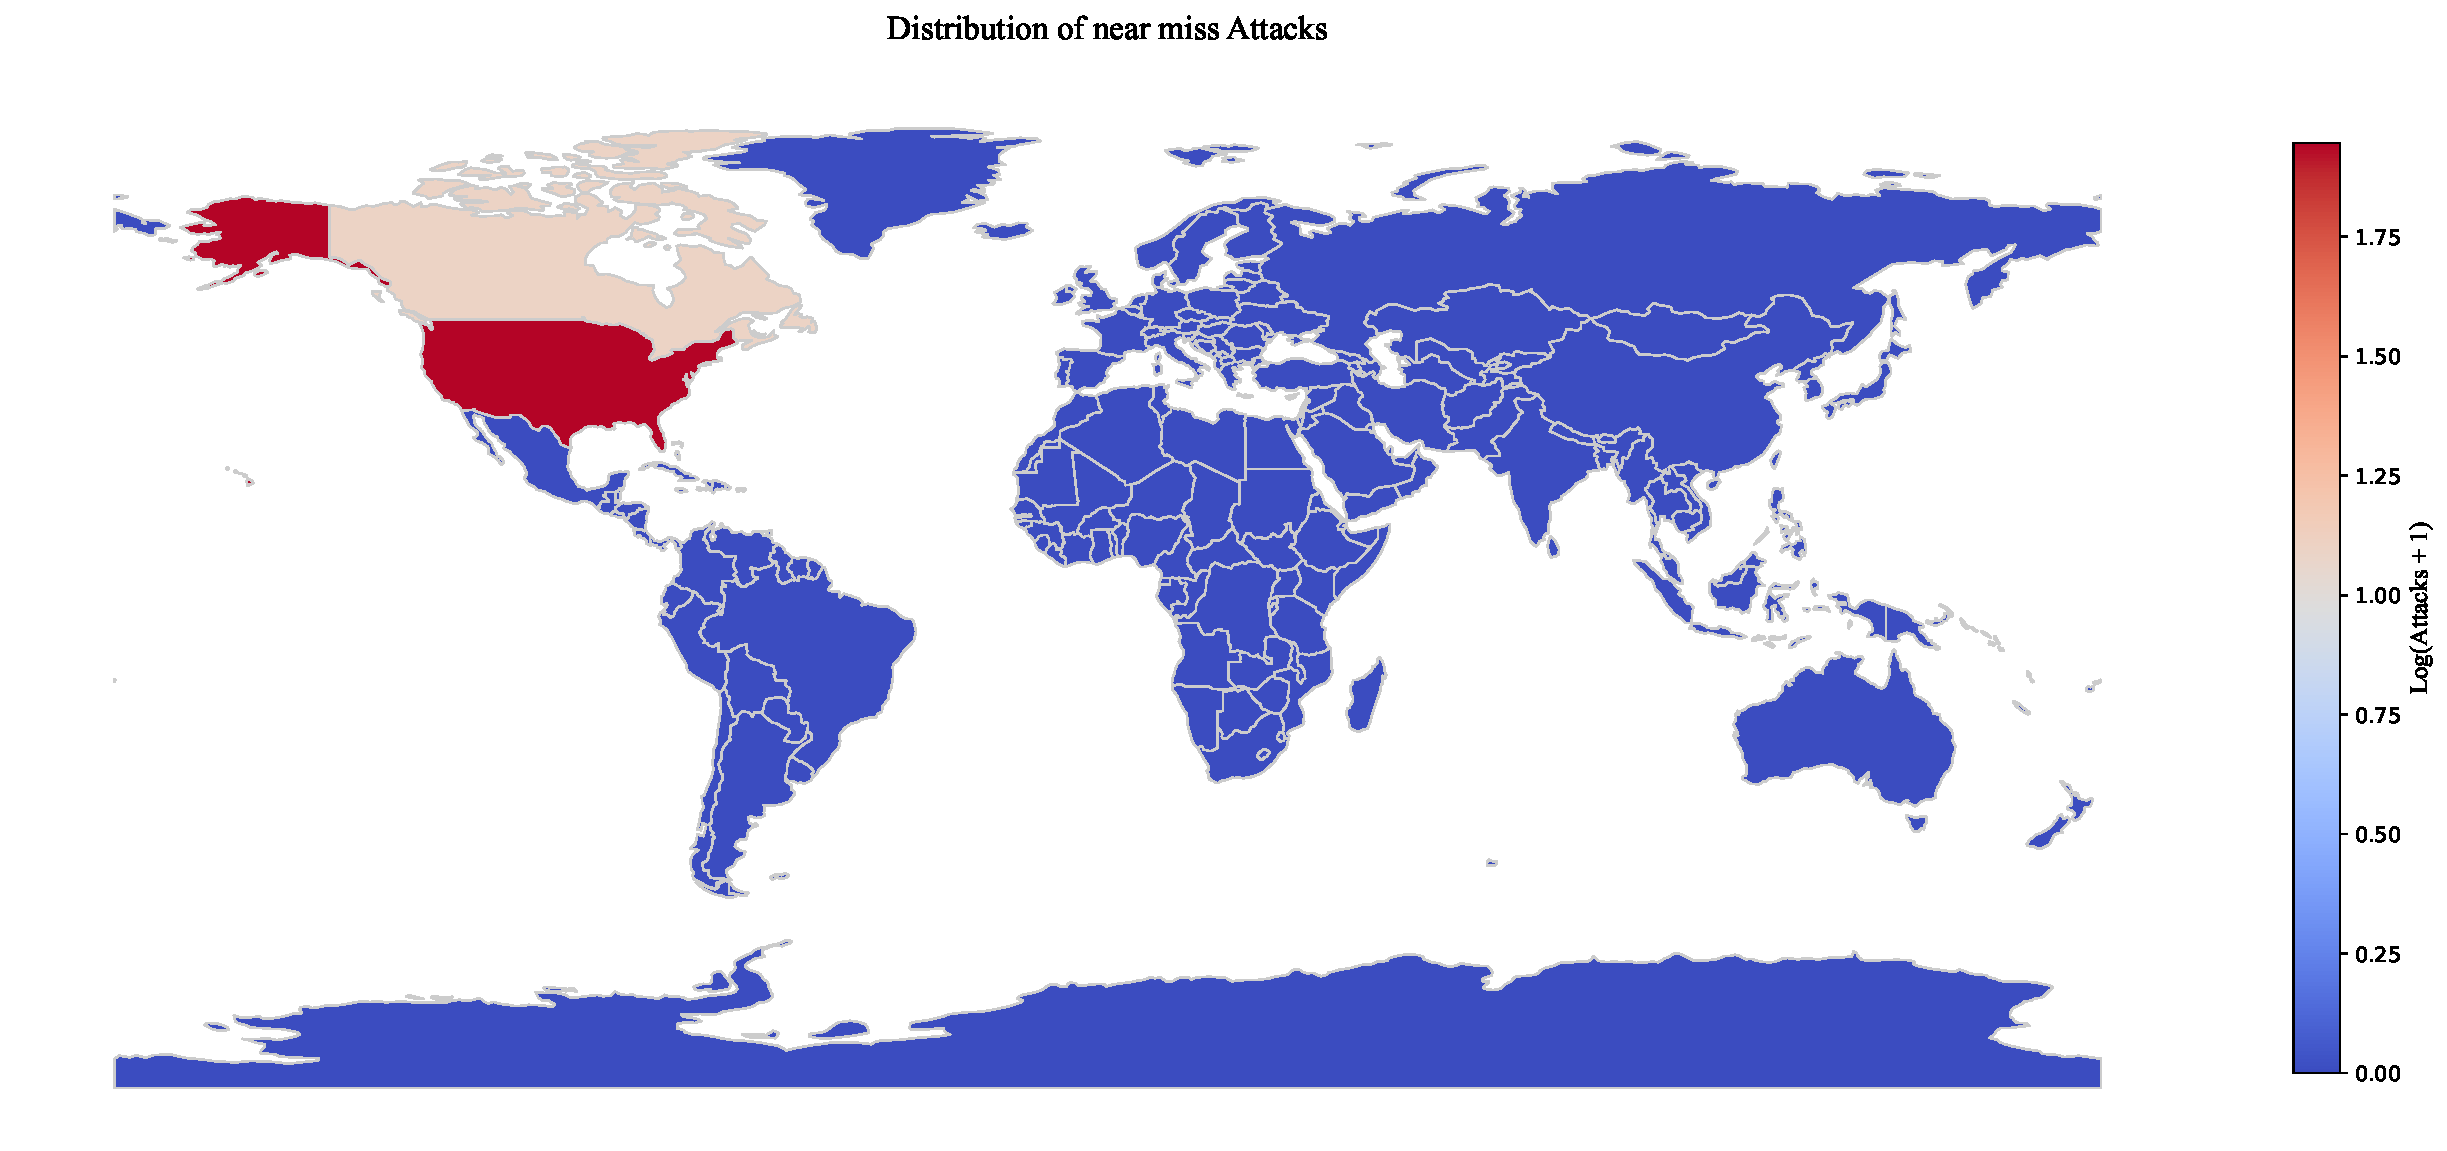
\includegraphics[scale=0.33]{./rsrc/Crime_NearMiss_distribution}
		}
		\quad
		\subfigure[Reported Cybercrime Incidents]{
			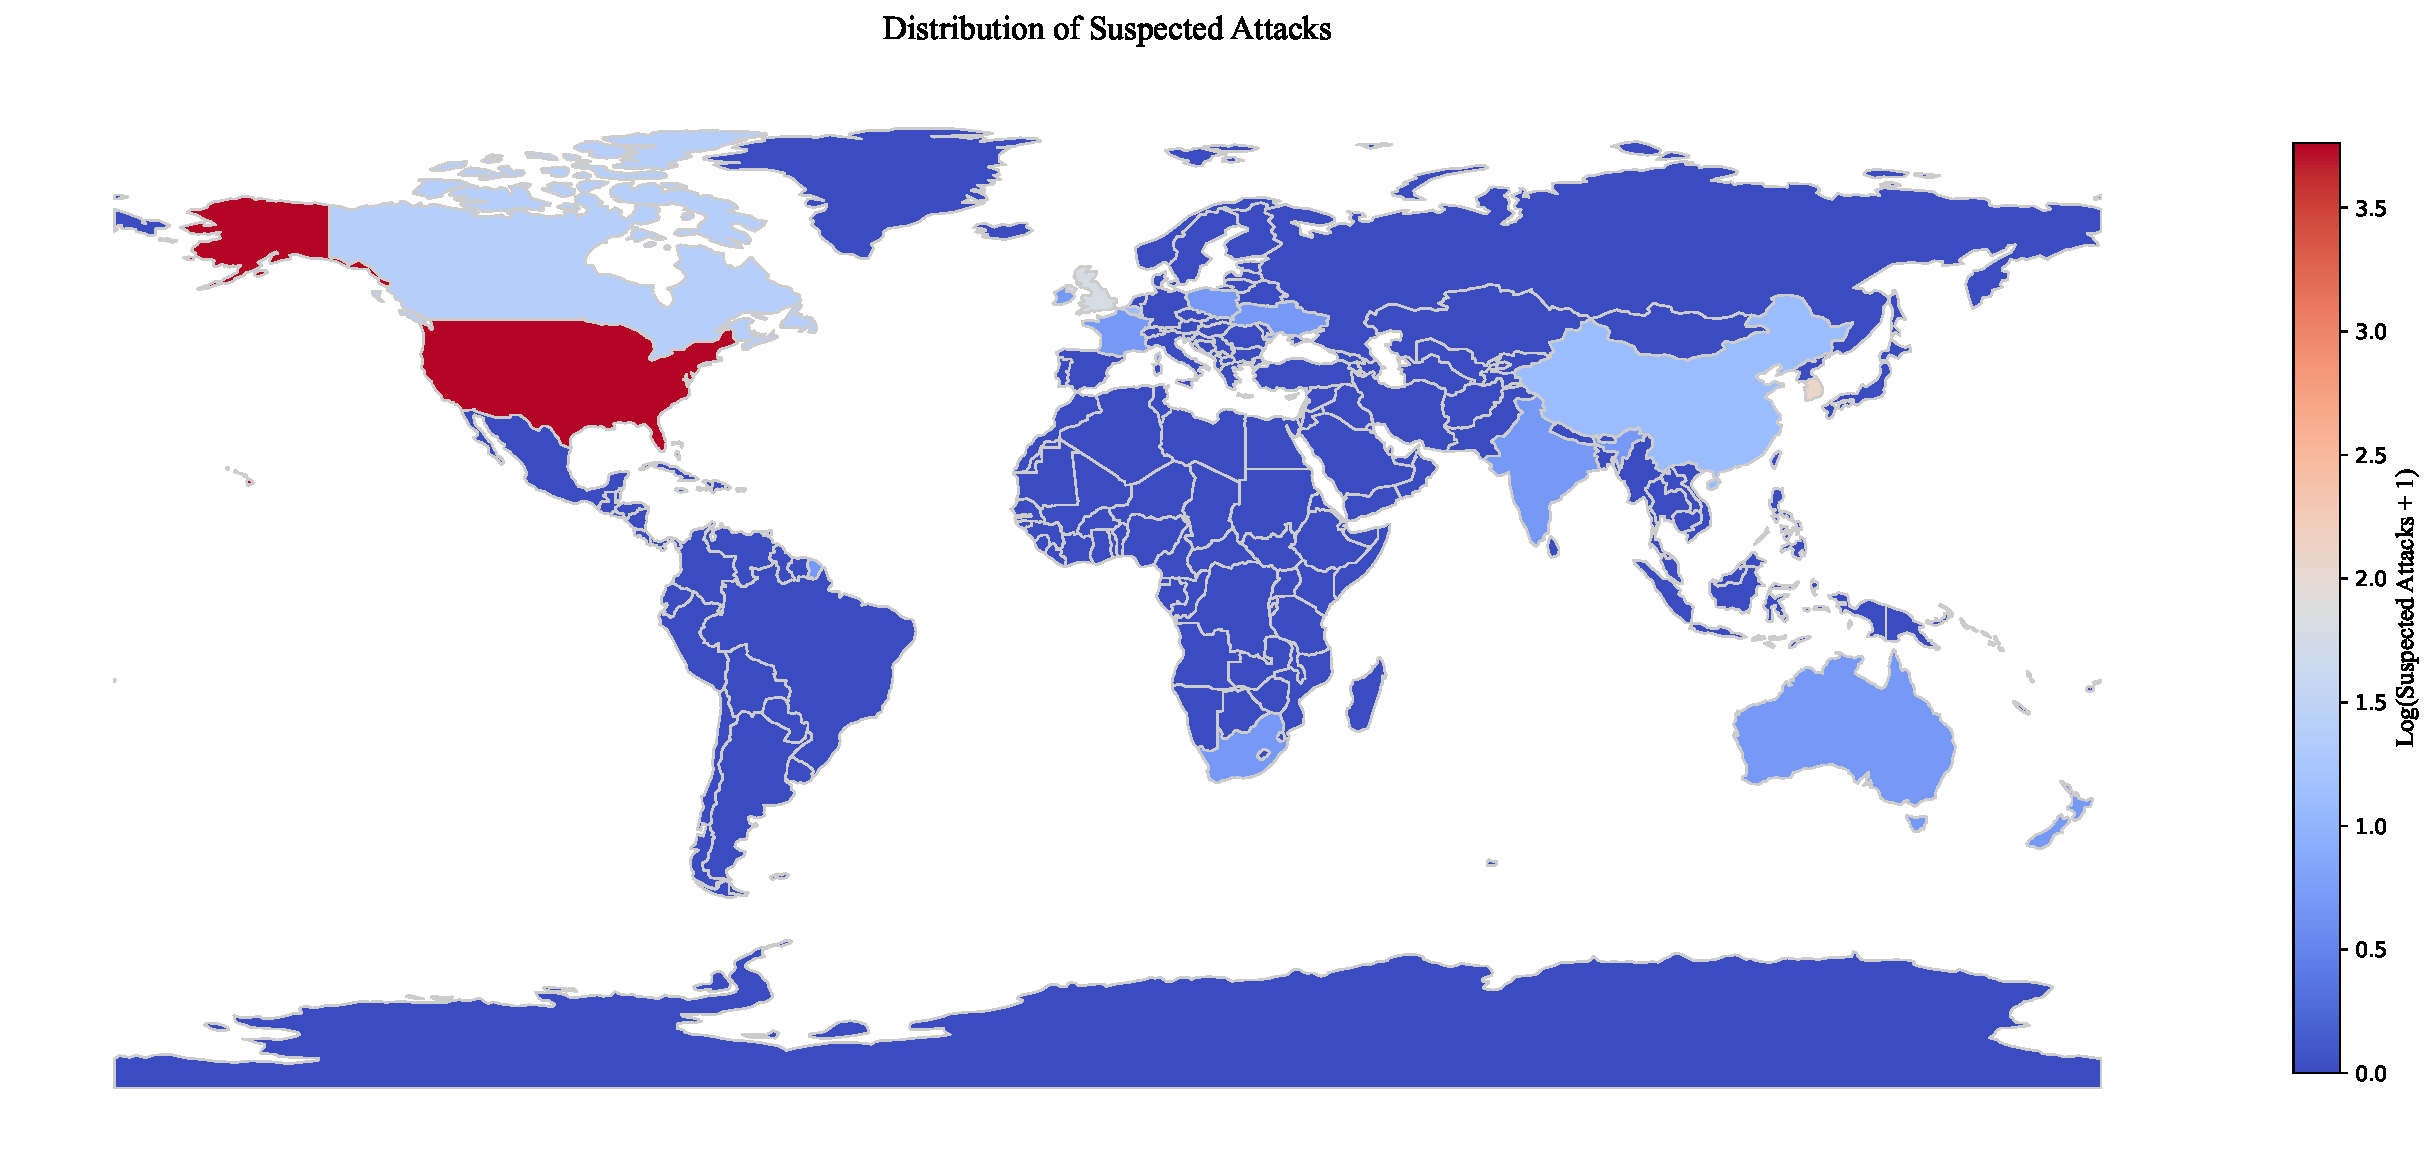
\includegraphics[scale=0.33]{./rsrc/Crime_Suspected_distribution}
		}
		\caption{Other Cybercrime Incidents}\label{fig:other-cybercrime-incidents}
	\end{figure}